\subsection{形式光滑代数}

设 \(k\) 为环，A 为 \(k\)-线性拓扑代数 (III, § 4, 第 2 节, 定义 1)。

定义 1. 我们称 A 在 k 上形式光滑，或称 A 为形式光滑 k-代数，如果它满足下述条件：对每个 k-代数 C 与 C 的每个平方零理想 N，从 A 到赋予离散拓扑的 k-代数 C/N 的每个连续同态都可提升为从 A 到赋予离散拓扑的 k-代数 C 的连续同态。

回忆：从 A 到赋予离散拓扑的 \(k\)-代数中的同态是连续的，当且仅当其核是开的。

设 \(k\) 为环，A 为线性拓扑的形式光滑 \(k\)-代数，J 为 A 的理想。赋予 A 以 J-进拓扑。设 C 为 \(k\)-代数，N 为 C 中的平方零理想；赋予 C 与 C/N 以离散拓扑。设 \(\varphi : A \to C/N\) 为连续代数同态。任何提升 \(\tilde{\varphi} : A \to C\)（\(\varphi\) 的提升）都是连续的：事实上，存在整数 \(n\) 使 \(\varphi(J^n)\) 为零，而我们有 \(\tilde{\varphi}(J^n) \subset N\)，从而 \(\tilde{\varphi}(J^{2n}) \subset N^2 = 0\)。特别由此推出：若 A 对 J-进拓扑形式光滑，则对包含 J 的每个理想 J′，它对 J′-进拓扑也形式光滑。

我们将称 \(k\)-代数 A 是形式光滑的，如果它被赋予离散拓扑（即 (0)-进拓扑）时形式光滑；于是它对 A 的任何理想 J 的 J-进拓扑都形式光滑。

注.- 1) 设 \(k\) 为环，A 为线性拓扑的形式光滑 \(k\)-代数，J 为 A 的理想。若 \(k\)-代数 A/J（对离散拓扑）形式光滑，则 A/J 的恒同映射可提升到 \(\mathrm{A} / \mathrm{J}^2\)；于是命题 2 中所述的那些集合非空。特别地，序列

\[
0 \to J / J ^ {2} \xrightarrow {\bar {d}} (A / J) \otimes_ {A} \Omega_ {k} (A) \longrightarrow \Omega_ {k} (A / J) \to 0
\]

是正合的且分裂的。

\begin{enumerate}
\def\labelenumi{\arabic{enumi})}
\setcounter{enumi}{1}
\tightlist
\item
  设 \(k\) 为环，\(\Lambda\) 为线性拓扑的形式光滑 \(k\)-代数，M 为零化子在 A 中是开集的 A-模。则每个导子 \(\delta\)（\(k\) 到 M 中的）都可扩张为从 A 到 M 中的导子。事实上，令 B = A/Ann(M)；映射 \(\lambda \mapsto (\lambda 1_{B}, \delta(\lambda))\) 定义了从 \(k\) 到 B ⊕ M 中的环同态 (第 1 节, 例)，也就是 B ⊕ M 上的一个 \(k\)-代数结构。典范满射 \(\varphi: A \to B\) 连续，故有提升 \(\tilde{\varphi}: A \to B \oplus M\)；据同上引文，pr \(_{2}\) \(\circ\) \(\tilde{\varphi}\) 是 \(\Lambda\) 到 M 中的导子且扩张 \(\delta\)。
\end{enumerate}

命题 3. - 设 k 为环。

\begin{enumerate}
\def\labelenumi{\alph{enumi})}
\item
  设 A 与 B 为线性拓扑 k-代数，\(\mathfrak{p}: \mathrm{A} \to \mathrm{B}\) 为连续 k-代数同态。若 A 在 \(k\) 上形式光滑且 B 在 A 上形式光滑，则 B 在 \(k\) 上形式光滑。
\item
  有限族线性拓扑的形式光滑 k-代数的乘积 k-代数是形式光滑的。
\item
  设 A 为 \(k\)-线性拓扑代数，\(\hat{\Lambda}\) 为 A 的分离完备化；为使 A 在 \(k\) 上形式光滑，必须且只需 \(\hat{\Lambda}\) 如此。
\end{enumerate}

设 C 为 \(k\)-代数，A 为 C-代数，N 为 C 中的平方零理想，\(\pi : \mathrm{C} \to \mathrm{C/N}\) 为典范满射。赋予 C 与 C/N 以离散拓扑。

\begin{enumerate}
\def\labelenumi{\alph{enumi})}
\tightlist
\item
  设 \(\psi : B \to C/N\) 为连续 \(k\)-代数同态。由于 A 在 \(k\) 上形式光滑，存在连续 \(k\)-代数同态 \(\tilde{\varphi} : A \to C\) 使 \(\pi \circ \tilde{\varphi} = \psi \circ \rho\)。
\end{enumerate}

\pandocbounded{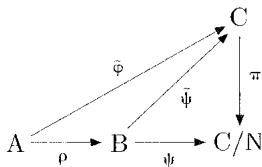
\includegraphics[keepaspectratio]{images/part001_4eedc660.jpg}}

借助 \(\tilde{\varphi}\) 把 C 与 C/N 视为 A-代数，于是 \(\psi\) 是 \(A\) -代数同态；由于 B 在 A 上形式光滑，存在连续 A-代数同态 \(\tilde{\psi}: B \to C\) 使 \(\pi \circ \tilde{\psi} = \psi\)，由此得 a)。

\begin{enumerate}
\def\labelenumi{\alph{enumi})}
\setcounter{enumi}{1}
\item
  只需证明两个形式光滑 \(k\)-代数 \(\mathrm{A}_1\) 与 \(\mathrm{A}_2\) 的乘积形式光滑。设 \(\varphi : \mathrm{A}_1 \times \mathrm{A}_2 \to \mathrm{C} / \mathrm{N}\) 为连续 \(k\)-代数同态。令 \(e_1 = \varphi(1,0)\)，\(e_2 = \varphi(0,1)\)，于是 \(e_1\) 与 \(e_2\) 是 \(\mathrm{C} / \mathrm{N}\) 中的正交幂等元。设 \(\varphi_1 : \mathrm{A}_1 \to (\mathrm{C} / \mathrm{N})e_1\) 与 \(\varphi_2 : \mathrm{A}_2 \to (\mathrm{C} / \mathrm{N})e_2\) 为由 \(\varphi_1(a_1) = \varphi(a_1,0)\) 与 \(\varphi_2(a_2) = \varphi(0,a_2)\) 定义的映射；它们是连续 \(k\)-代数同态，且有 \(\varphi(a_1,a_2) = \varphi_1(a_1) + \varphi_2(a_2)\)（对每个 \((a_1,a_2) \in \mathrm{A}_1 \times \mathrm{A}_2\)）。存在 C 的幂等元 \(\tilde{e}_1\) 使 \(\pi(\tilde{e}_1) = e_1\) (A, VIII, § 9, 第 4 节, 命题 7)；令 \(\tilde{e}_2 = 1 - \tilde{e}_1\)，于是 \(\pi(\tilde{e}_2) = e_2\)。为证这对 \(i = 1,2\) 成立：同态 \(\mathrm{C}\tilde{e}_i \to (\mathrm{C} / \mathrm{N})e_i\)（由 \(\pi\) 诱导）是满射的，核为 \(\mathrm{N}\tilde{e}_i\)；由于 \(k\)-代数 \(\mathrm{A}_i\) 形式光滑，同态 \(\varphi_i\) 有一个连续提升 \(\tilde{\varphi}_i\)（到 \(\mathrm{C}\tilde{e}_i\) 中）。映射 \((a_1,a_2) \mapsto \tilde{\varphi}_1(a_1) + \tilde{\varphi}_2(a_2)\) 是 \(\varphi\) 到 C 中的连续提升。
\item
  设 \(i: \mathrm{A} \to \widehat{\mathrm{A}}\) 为典范同态。对每个赋予离散拓扑的环 D，把连续同态 \(f: \widehat{\mathrm{A}} \to \mathrm{D}\) 对应为连续同态 \(f \circ i: \mathrm{A} \to \mathrm{D}\) 的映射是双射的。断言 c) 由此得出。
\end{enumerate}

命题的断言 c) 特别适用于 \(A\) 的拓扑是 J-进拓扑且 \(J\) 是有限生成理想的情形：此时闭包 \(\widehat{J}\)（\(J\) 在 \(\widehat{A}\) 中的）等于 \(\widehat{JA}\)，且 \(\widehat{A}\) 的拓扑是 \(\widehat{J}\)-进拓扑 (III, § 2, 第 12 节, 命题 16 的推论 2)。于是，说 \(A\) 对 J-进拓扑形式光滑，与说它的分离完备化 \(\widehat{A}\) 对 J-进拓扑形式光滑，两者等价。

命题 4.--- 设 k 为环，A 与 B 为 k-代数，J 为 A 的理想，K 为 B 的理想。

\begin{enumerate}
\def\labelenumi{\alph{enumi})}
\item
  设 S 为 A 的乘性子集，T 为 k 的其在 A 中的像含于 S 的子集。若 \(A\) 对 J-进拓扑在 \(k\) 上形式光滑，则 S \(^{-1}A\) 在 \(\mathrm{T}^{-1}k\) 上对 \(\mathrm{S}^{-1}\mathrm{J}\)-进拓扑形式光滑。
\item
  设 \(k'\) 为 \(k\)-代数。若 A 对 J-进拓扑在 \(k\) 上形式光滑，则 \(k'\)-代数 \(A_{(k')}\) 在 \(k'\) 上对 \(JA_{(k')}\)-进拓扑形式光滑。
\item
  以 I 表示 A ⊗k B 中由 J ⊗k B 与 A ⊗k K 的像生成的理想。若 A 与 B 分别对 J-进与 K-进拓扑在 k 上形式光滑，则 k-代数 A ⊗k B 对 I-进拓扑形式光滑。
\item
  在 a) 的假设下，设 C 为 \(\mathrm{T}^{-1}k\)-代数，N 为 C 中的平方零理想；赋予 C 与 C/N 以离散拓扑，并以 \(\pi : C \to C/N\) 表示典范满射。设 \(\varphi : S^{-1}A \longrightarrow C/N\) 为一个 \(\mathrm{T}^{-1}k\)-代数同态（对 \(\mathrm{S}^{-1}\mathrm{J}\)-进拓扑连续）。以 i 表示从 A 到 \(S^{-1}A\) 中的典范同态。映射 \(\varphi \circ i\) 是对 J-进拓扑连续的 k-代数同态，故有提升 \(\tilde{\varphi}_{0} : A \to C\)。\(\tilde{\varphi}_{0}(S)\) 中的元素模 N 可逆，由于 N 幂零，故它们可逆。于是存在环同态 \(\tilde{\varphi} : S^{-1}A \to C\) 使 \(\tilde{\varphi} \circ i = \tilde{\varphi}_{0}\) (II, § 2, 第 1 节, 命题 1)；由同上引文命题 2 的推论 3，\(\tilde{\varphi}\) 是 \(\mathrm{T}^{-1}k\)-线性的。我们有 \(\pi \circ \tilde{\varphi} \circ i = \varphi \circ i\)，从而 \(\pi \circ \tilde{\varphi} = \varphi\) (同上引文, 命题 1)，于是 \(\tilde{\varphi}\) 是 \(\varphi\) 的一个提升。
\item
  置身于 b) 的假设之下。设 C 为 \(k'\)-代数，N 为 C 中的平方零理想；赋予 C 与 C/N 以离散拓扑。设 \(\varphi : \mathrm{A}_{(k')} \longrightarrow \mathrm{C/N}\) 为一个 \(k'\)-代数同态（对 \(J\mathrm{A}_{(k')}\)-进拓扑连续）。以 \(i : \mathrm{A} \to \mathrm{A}_{(k')}\) 表示典范同态。映射 \(\varphi \circ i\) 是从 A 到 C/N 的、对 J-进拓扑连续的 \(k\)-代数同态；若 A 对 J-进拓扑在 \(k\) 上形式光滑，则 \(\varphi \circ i\) 有提升 \(\tilde{\psi} : \mathrm{A} \to \mathrm{C}\)。\(k'\)-代数同态 \(\tilde{\varphi} : \mathrm{A}_{(k')} \longrightarrow \mathrm{C}\)（由 \(\tilde{\psi}\) 导出）是 \(\varphi\) 的一个提升。
\item
  置身于 c) 的假设之下。由 b)，B-代数 A⊗ \(_{k}\) B 对 J(A⊗ \(_{k}\) B)-进拓扑形式光滑，从而对 I-进拓扑形式光滑；此外，当 B 赋予 K-进拓扑且 A⊗ \(_{k}\) B 赋予 I-进拓扑时，典范同态 B → A⊗ \(_{k}\) B 连续。于是断言 c) 由命题 3, a) 得出。
\end{enumerate}

